\documentclass[11pt,letterpaper]{article}

\usepackage{fontspec}
\usepackage{babel}
\babelprovide[import,main]{spanish}
\setlocalecaption{spanish}{table}{Tabla}
\usepackage[margin=2.5cm]{geometry}
\usepackage{amsmath,amssymb,amsthm}
\usepackage{booktabs}
\usepackage{array}
\usepackage{float}
\usepackage[hidelinks]{hyperref}
% Paquetes, estilos y macros compartidos por las figuras
\usepackage{tikz}
\usetikzlibrary{arrows.meta,positioning,calc}

\tikzset{
  flecha/.style={-{Stealth[length=2.2mm]}, thick},
  caja/.style={draw, thick, align=center, minimum height=1.25cm, text width=3.2cm, font=\small},
  obs/.style={circle, fill=black, inner sep=0pt, minimum size=1.5mm},
  muestra/.style={rectangle, draw, thick, fill=white, inner sep=0pt, minimum size=2.1mm},
  hueco/.style={circle, draw=black!60, fill=white, inner sep=0pt, minimum size=1.5mm},
}

% Imagen de 16 x 16 píxeles de una lata: x, y, anchura y altura en píxeles
\newcommand{\lata}[4]{%
  \begin{scope}[shift={(#1,#2)},x=0.09cm,y=0.09cm]
    \pgfmathtruncatemacro{\lizq}{(16-#3)/2}
    \pgfmathtruncatemacro{\lder}{\lizq+#3}
    \pgfmathtruncatemacro{\ltope}{2+#4}
    \pgfmathtruncatemacro{\lborde}{\ltope-2}
    \fill[black!7] (0,0) rectangle (16,16);
    \fill[black!58] (\lizq,2) rectangle (\lder,\ltope);
    \fill[black!30] (\lizq,\lborde) rectangle (\lder,\ltope);
    \fill[black!78] (\lizq,2) rectangle (\lder,3);
    \draw[white, line width=0.15pt] (0,0) grid (16,16);
    \draw[black!60, line width=0.4pt] (0,0) rectangle (16,16);
  \end{scope}%
}


\setlength{\parindent}{0pt}
\setlength{\parskip}{0.6em}
\setlength{\emergencystretch}{3em}

\theoremstyle{definition}
\newtheorem{definicion}{Definición}

\newcommand{\bx}{\mathbf{x}}
\newcommand{\bz}{\mathbf{z}}
\newcommand{\bv}{\mathbf{v}}
\newcommand{\bh}{\mathbf{h}}
\newcommand{\bX}{\mathbf{X}}
\newcommand{\pdata}{p_{\text{data}}}
\newcommand{\ptheta}{p_{\theta}}
\newcommand{\normal}{\mathcal{N}}
\DeclareMathOperator*{\argmax}{arg\,max}

\newenvironment{referencias}
  {\begin{list}{}{\setlength{\leftmargin}{1.5em}\setlength{\itemindent}{-1.5em}\setlength{\itemsep}{0.3em}\setlength{\parsep}{0pt}}}
  {\end{list}}

\begin{document}

\begin{center}
  {\LARGE Fundamentos de los modelos generativos}
\end{center}
\vspace{0.5em}

%-------------------------------------------------------------
\section{Introducción}

La IA generativa es un conjunto de algoritmos y modelos capaces de producir contenido nuevo, como texto, imágenes, video, código o estrategias, con una creatividad y adaptabilidad parecidas a las humanas (He et al., 2025).

Su base es el modelo generativo, que describe mediante un modelo probabilístico cómo se genera un conjunto de datos, de modo que al muestrear de él se obtienen datos nuevos (Foster, 2019).

En otras palabras, un modelo generativo busca capturar la distribución que genera una clase de datos para producir datos similares (Oussidi y Elhassouny, 2018).

Las arquitecturas profundas, con muchas capas no lineales y variables latentes, permiten aprender representaciones complejas a partir de grandes cantidades de datos sin etiquetar (Salakhutdinov, 2015).

Entre los modelos principales, descritos por Salakhutdinov (2015), Oussidi y Elhassouny (2018) y He et al. (2025), se encuentran las máquinas de Boltzmann, los autocodificadores variacionales, las redes generativas adversarias, los modelos autorregresivos, los modelos de difusión y los transformers.

Los retos de esta área incluyen las alucinaciones, el costo y el uso indebido (He et al., 2025).

Este documento profundiza en la definición formal de los modelos generativos, sus componentes, el espacio latente y su contraste con los modelos discriminativos, y deja para una etapa posterior el estudio de cada modelo en particular.

%-------------------------------------------------------------
\section{Definición formal}

Se parte de un conjunto de observaciones $\bX = \{\bx_1, \dots, \bx_N\}$, llamado datos de entrenamiento, donde cada $\bx_i$ pertenece a un espacio muestral $\mathcal{X} \subseteq \mathbb{R}^d$, que es el conjunto de todos los valores que puede tomar una observación (Foster, 2019).

En un problema de imágenes, las características de cada observación suelen ser los valores de sus píxeles, por lo que la dimensión $d$ es alta (Foster, 2019).

Se supone que las observaciones fueron generadas de forma independiente por una distribución desconocida $\pdata$ (Foster, 2019).

\begin{definicion}[Modelo generativo]
Un modelo generativo es un modelo probabilístico $\ptheta$ que describe cómo se genera un conjunto de datos, de modo que imita a $\pdata$ y al muestrear de él se obtienen datos nuevos.
\end{definicion}

La Figura~\ref{fig:proceso} resume este proceso.

\begin{figure}[H]
  \centering
  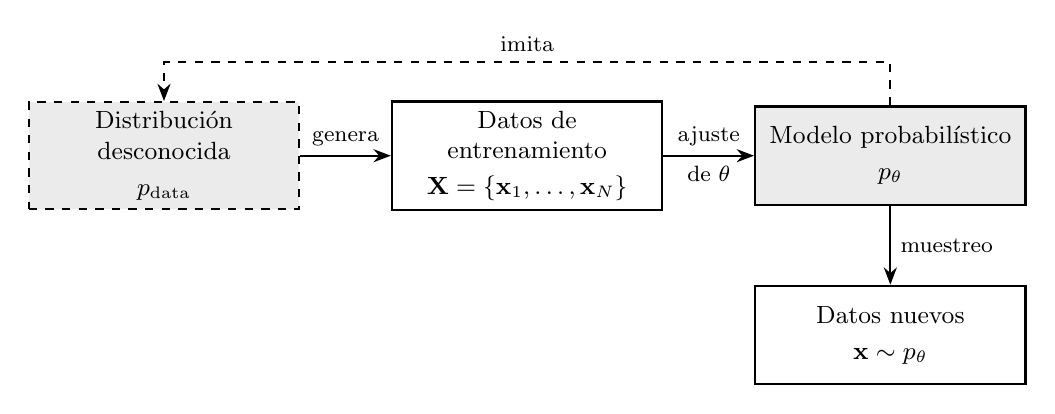
\begin{tikzpicture}[node distance=1.15cm]
  \node[caja, fill=black!8, dashed] (pdata) {Distribución desconocida\\[2pt] $\pdata$};
  \node[caja, right=of pdata] (datos) {Datos de entrenamiento\\[2pt] \mbox{$\bX = \{\bx_1, \dots, \bx_N\}$}};
  \node[caja, right=of datos, fill=black!8] (modelo) {Modelo probabilístico\\[2pt] $\ptheta$};
  \node[caja, below=1.0cm of modelo] (nuevos) {Datos nuevos\\[2pt] \mbox{$\bx \sim \ptheta$}};
  \draw[flecha] (pdata) -- node[above, font=\footnotesize] {genera} (datos);
  \draw[flecha] (datos) -- node[above, font=\footnotesize] {ajuste} node[below, font=\footnotesize] {de $\theta$} (modelo);
  \draw[flecha] (modelo) -- node[right, font=\footnotesize] {muestreo} (nuevos);
  \draw[flecha, dashed] (modelo.north) -- ++(0,0.55) -| node[pos=0.25, above, font=\footnotesize] {imita} (pdata.north);
\end{tikzpicture}

  \caption{Un modelo generativo se ajusta a partir de observaciones de una distribución desconocida, la imita y permite muestrear datos nuevos}
  \label{fig:proceso}
\end{figure}

El modelo es paramétrico cuando es una familia de funciones de densidad $\ptheta(\bx)$ descrita por un número finito de parámetros $\theta$ (Foster, 2019).

La verosimilitud mide qué tan plausibles son los valores de $\theta$ dados los datos y, para observaciones independientes, se define como (Foster, 2019)
\begin{equation}
  \mathcal{L}(\theta \mid \bX) = \prod_{\bx \in \bX} \ptheta(\bx).
\end{equation}

Como este producto es difícil de calcular, se suele trabajar con su logaritmo,
\begin{equation}
  \ell(\theta \mid \bX) = \sum_{\bx \in \bX} \log \ptheta(\bx).
\end{equation}

La estimación por máxima verosimilitud busca los parámetros que hacen más probable observar los datos (Foster, 2019),
\begin{equation}
  \hat{\theta} = \argmax_{\theta} \ell(\theta \mid \bX).
\end{equation}

El modelo debe ser probabilístico y no determinista, ya que un cálculo fijo, como el promedio de cada píxel, produce siempre la misma salida (Foster, 2019).

Un modelo generativo es bueno si sus muestras parecen provenir de $\pdata$ y además son suficientemente distintas de los datos de entrenamiento (Foster, 2019).

Por la segunda condición, el modelo no debe limitarse a reproducir lo que ya vio (Foster, 2019).

La Figura~\ref{fig:muestras} ilustra estas dos condiciones.

\begin{figure}[H]
  \centering
  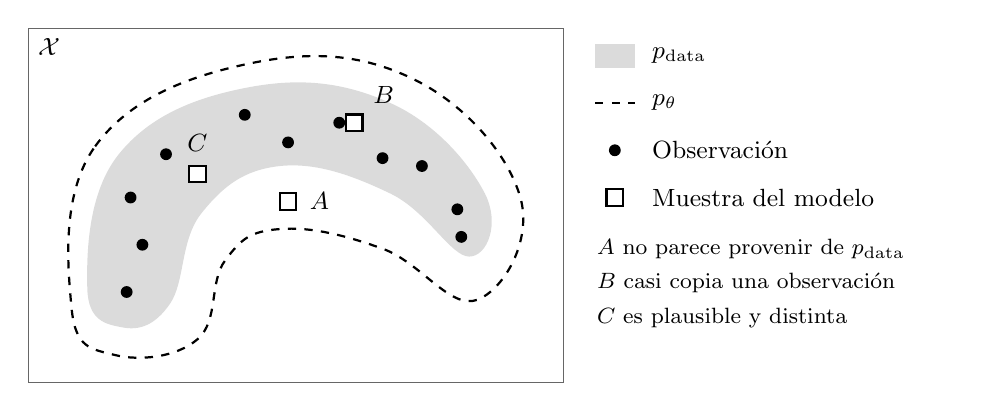
\begin{tikzpicture}
  \draw[black!60] (0,0) rectangle (6.8,4.5);
  \node[anchor=north west, font=\small] at (0,4.5) {$\mathcal{X}$};
  % Distribución real
  \fill[black!14] plot[smooth cycle, tension=0.7] coordinates
    {(0.75,1.2) (1.15,2.9) (2.8,3.75) (4.6,3.55) (5.8,2.4) (5.6,1.6) (4.6,2.4) (3.2,2.75) (2.2,2.15) (1.8,1.0) (1.2,0.7)};
  % Modelo
  \draw[thick, dashed] plot[smooth cycle, tension=0.7] coordinates
    {(0.55,0.95) (0.85,3.0) (2.8,4.05) (4.9,3.85) (6.25,2.35) (5.7,1.05) (4.5,1.7) (3.2,1.95) (2.5,1.55) (2.15,0.55) (1.1,0.35)};
  % Observaciones
  \foreach \p in {(1.25,1.15),(1.45,1.75),(1.3,2.35),(1.75,2.9),(2.75,3.4),(3.3,3.05),(3.95,3.3),(4.5,2.85),(5.0,2.75),(5.45,2.2),(5.5,1.85)}
    \node[obs] at \p {};
  % Muestras
  \node[muestra] (A) at (3.3,2.3) {};
  \node[font=\small, right=1pt of A] {$A$};
  \node[muestra] (B) at (4.14,3.3) {};
  \node[font=\small, above right=0pt of B] {$B$};
  \node[muestra] (C) at (2.15,2.65) {};
  \node[font=\small, above=1pt of C] {$C$};
  % Leyenda
  \begin{scope}[shift={(7.2,0.25)}, font=\small]
    \fill[black!14] (0,3.75) rectangle (0.5,4.05);
    \node[anchor=west] at (0.6,3.9) {$\pdata$};
    \draw[thick, dashed] (0,3.3) -- (0.5,3.3);
    \node[anchor=west] at (0.6,3.3) {$\ptheta$};
    \node[obs] at (0.25,2.7) {};
    \node[anchor=west] at (0.6,2.7) {Observación};
    \node[muestra] at (0.25,2.1) {};
    \node[anchor=west] at (0.6,2.1) {Muestra del modelo};
    \node[anchor=north west, text width=4.5cm, align=left, font=\footnotesize] at (-0.1,1.7)
      {$A$ no parece provenir de $\pdata$\\[3pt] $B$ casi copia una observación\\[3pt] $C$ es plausible y distinta};
  \end{scope}
\end{tikzpicture}

  \caption{El modelo $\ptheta$ aproxima a $\pdata$ y una buena muestra, como $C$, parece real sin copiar los datos de entrenamiento, con base en las reglas de Foster (2019)}
  \label{fig:muestras}
\end{figure}

Según el tratamiento de la densidad, algunos modelos la definen de forma explícita, como PixelRNN y los autocodificadores variacionales, mientras que otros la definen de forma implícita, como las redes generativas adversarias (Oussidi y Elhassouny, 2018).

%-------------------------------------------------------------
\section{Componentes}

Un modelo generativo profundo con variables latentes se compone de los siguientes elementos.

\begin{itemize}
  \item \textbf{Datos de entrenamiento:} las observaciones de $\bX$, que son el único acceso disponible a $\pdata$ (Foster, 2019).
  \item \textbf{Variable latente:} un vector $\bz$ no observado que representa cada dato en un espacio de menor dimensión (Foster, 2019).
  \item \textbf{Distribución a priori:} una distribución $p(\bz)$ de la que se puede muestrear, como la normal estándar en los autocodificadores variacionales (Foster, 2019).
  \item \textbf{Generador:} una función aprendida por una red profunda que lleva cada punto del espacio latente al espacio de los datos (Foster, 2019).
  \item \textbf{Función objetivo:} el criterio que guía el aprendizaje, como la verosimilitud (Foster, 2019), una cota inferior de esta (Salakhutdinov, 2015) o un juego minimax (Oussidi y Elhassouny, 2018).
\end{itemize}

Una vez entrenado el modelo, generar un dato nuevo consiste en muestrear primero un valor latente y después un dato condicionado a ese valor,
\begin{equation}
  \bz \sim p(\bz), \qquad \bx \sim \ptheta(\bx \mid \bz).
\end{equation}

%-------------------------------------------------------------
\section{Espacio latente}

\subsection{Idea general}

De todas las formas posibles de asignar valores a los píxeles, solo una parte muy pequeña corresponde a imágenes de la entidad que se quiere simular (Foster, 2019).

Por ello, en lugar de modelar directamente el espacio de alta dimensión, se describe cada observación con un espacio latente de baja dimensión y se aprende una función que lleve cada punto de ese espacio al dominio original (Foster, 2019).

Por ejemplo, un conjunto de imágenes en escala de grises de latas de galletas se puede representar con solo dos características, la altura y la anchura de cada lata (Foster, 2019).

\begin{definicion}[Espacio latente]
El espacio latente es un espacio $\mathcal{Z} \subseteq \mathbb{R}^k$, con $k \ll d$, cuyos puntos $\bz$ son representaciones de baja dimensión de las observaciones.
\end{definicion}

La Figura~\ref{fig:latas} ilustra esta definición con el ejemplo de las latas.

\begin{figure}[H]
  \centering
  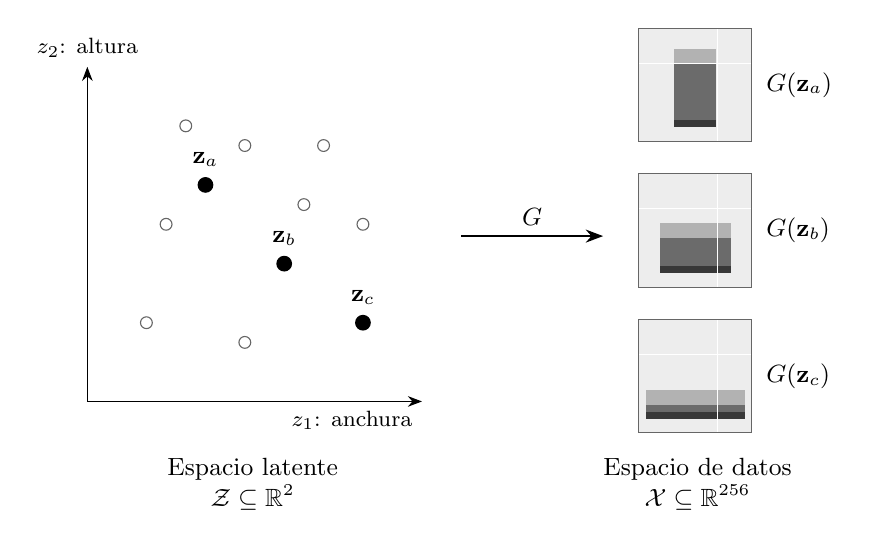
\begin{tikzpicture}
  % Plano latente
  \begin{scope}[x=0.25cm,y=0.25cm]
    \draw[-{Stealth[length=1.8mm]}] (0,0) -- (17,0) node[below left, font=\footnotesize] {$z_1$: anchura};
    \draw[-{Stealth[length=1.8mm]}] (0,0) -- (0,17) node[above, font=\footnotesize] {$z_2$: altura};
    \foreach \p in {(3,4),(4,9),(5,14),(8,3),(8,13),(11,10),(12,13),(14,9)}
      \node[hueco] at \p {};
    \node[obs, minimum size=2mm, label={[font=\small]above:$\bz_a$}] at (6,11) {};
    \node[obs, minimum size=2mm, label={[font=\small]above:$\bz_b$}] at (10,7) {};
    \node[obs, minimum size=2mm, label={[font=\small]above:$\bz_c$}] at (14,4) {};
  \end{scope}
  \node[font=\small, align=center] at (2.1,-1.05) {Espacio latente\\ $\mathcal{Z} \subseteq \mathbb{R}^{2}$};
  % Generador
  \draw[flecha] (4.75,2.1) -- node[above, font=\small] {$G$} (6.55,2.1);
  % Imágenes
  \lata{7}{3.3}{6}{11}
  \lata{7}{1.45}{10}{7}
  \lata{7}{-0.4}{14}{4}
  \node[font=\small, right] at (8.5,4.02) {$G(\bz_a)$};
  \node[font=\small, right] at (8.5,2.17) {$G(\bz_b)$};
  \node[font=\small, right] at (8.5,0.32) {$G(\bz_c)$};
  \node[font=\small, align=center] at (7.75,-1.05) {Espacio de datos\\ $\mathcal{X} \subseteq \mathbb{R}^{256}$};
\end{tikzpicture}

  \caption{Cada imagen de $16 \times 16$ píxeles tiene $d = 256$ valores, pero se puede describir con $k = 2$ variables latentes, la anchura y la altura de la lata, con base en el ejemplo de Foster (2019)}
  \label{fig:latas}
\end{figure}

En términos matemáticos, se busca la variedad no lineal sobre la que se encuentran los datos y las dimensiones necesarias para describirla (Foster, 2019), como se muestra en la Figura~\ref{fig:variedad}.

\begin{figure}[H]
  \centering
  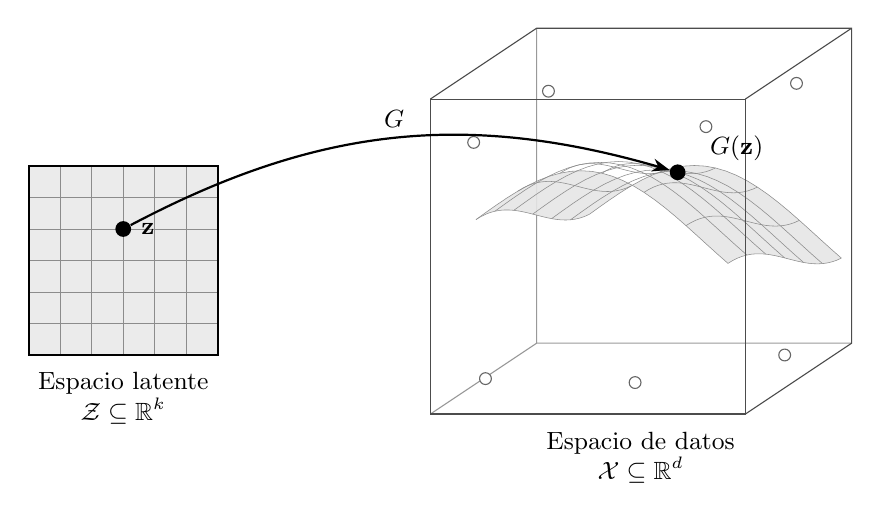
\begin{tikzpicture}[
  declare function={
    sx(\u,\v) = 0.4+3.2*\u + 0.45*(0.4+3.2*\v);
    sy(\u,\v) = 1.9 + 0.75*sin(200*\u) + 0.45*cos(170*\v) - 0.3*\u + 0.3*(0.4+3.2*\v);
  }]
  % Plano latente
  \begin{scope}[shift={(-5.1,0.75)}]
    \fill[black!8] (0,0) rectangle (2.4,2.4);
    \draw[black!45, step=0.4, very thin] (0,0) grid (2.4,2.4);
    \draw[thick] (0,0) rectangle (2.4,2.4);
    \node[obs, minimum size=2mm, label={[font=\small]right:$\bz$}] (z) at (1.2,1.6) {};
    \node[font=\small, align=center, below] at (1.2,-0.1) {Espacio latente\\ $\mathcal{Z} \subseteq \mathbb{R}^{k}$};
  \end{scope}
  % Cubo, aristas traseras
  \draw[black!40] (1.35,0.9) -- (5.35,0.9) (1.35,0.9) -- (1.35,4.9) (1.35,0.9) -- (0,0);
  % Superficie
  \fill[black!10, opacity=0.9]
    plot[domain=0:1, samples=25] ({sx(\x,0)},{sy(\x,0)}) --
    plot[domain=0:1, samples=25] ({sx(1,\x)},{sy(1,\x)}) --
    plot[domain=1:0, samples=25] ({sx(\x,1)},{sy(\x,1)}) --
    plot[domain=1:0, samples=25] ({sx(0,\x)},{sy(0,\x)}) -- cycle;
  \foreach \t in {0,1/6,2/6,3/6,4/6,5/6,1} {
    \draw[black!45, very thin] plot[domain=0:1, samples=25] ({sx(\x,\t)},{sy(\x,\t)});
    \draw[black!45, very thin] plot[domain=0:1, samples=25] ({sx(\t,\x)},{sy(\t,\x)});
  }
  % Cubo, aristas delanteras
  \draw[black!70] (0,0) rectangle (4,4);
  \draw[black!70] (4,0) -- (5.35,0.9) -- (5.35,4.9) -- (1.35,4.9) -- (0,4) (4,4) -- (5.35,4.9);
  % Puntos fuera de la variedad
  \foreach \p in {(0.55,3.45),(1.5,4.1),(3.5,3.65),(4.65,4.2),(0.7,0.45),(2.6,0.4),(4.5,0.75)}
    \node[hueco] at \p {};
  % Punto en la variedad
  \pgfmathsetmacro{\gx}{sx(0.5,0.667)}
  \pgfmathsetmacro{\gy}{sy(0.5,0.667)}
  \node[obs, minimum size=2mm] (gz) at (\gx,\gy) {};
  \node[font=\small] at ($(gz)+(0.75,0.3)$) {$G(\bz)$};
  \draw[flecha, bend left=22] (z) to node[above, font=\small] {$G$} (gz);
  \node[font=\small, align=center, below] at (2.67,-0.1) {Espacio de datos\\ $\mathcal{X} \subseteq \mathbb{R}^{d}$};
\end{tikzpicture}

  \caption{Los datos válidos se concentran en una variedad de baja dimensión dentro de $\mathbb{R}^{d}$, dibujado aquí en tres dimensiones, y $G$ lleva el espacio latente a esa variedad, con base en Foster (2019)}
  \label{fig:variedad}
\end{figure}

\subsection{Formulación}

La relación entre los datos y el espacio latente se expresa con la distribución conjunta,
\begin{equation}
  p(\bx, y) = p(\bx \mid y)\, p(y),
\end{equation}
donde $y$ es un valor del espacio latente, $p(y)$ es su distribución a priori y $p(\bx \mid y)$ es la distribución de los datos dado ese valor.

Para no confundir este valor con la etiqueta $y$ de los modelos discriminativos, en adelante se escribe $\bz$, como en Foster (2019) y Oussidi y Elhassouny (2018), de modo que
\begin{equation}
  \ptheta(\bx, \bz) = \ptheta(\bx \mid \bz)\, p(\bz).
\end{equation}

El modelo obtiene $\ptheta(\bx)$ al marginalizar la variable latente, con una suma si $\bz$ es discreta (Oussidi y Elhassouny, 2018) o con una integral si es continua,
\begin{equation}
  \ptheta(\bx) = \sum_{\bz} \ptheta(\bx \mid \bz)\, p(\bz), \qquad \ptheta(\bx) = \int_{\mathcal{Z}} \ptheta(\bx \mid \bz)\, p(\bz)\, d\bz.
  \label{eq:marginal}
\end{equation}

Esta expresión muestra la utilidad del espacio latente, porque la complejidad de los datos puede quedar a cargo de la función aprendida por la red profunda, que suele ser muy compleja (Foster, 2019).

El camino inverso lo da la distribución a posteriori, que indica qué valores latentes explican un dato observado,
\begin{equation}
  \ptheta(\bz \mid \bx) = \frac{\ptheta(\bx \mid \bz)\, p(\bz)}{\ptheta(\bx)}.
\end{equation}

El cálculo exacto en estos modelos suele ser intratable o demasiado costoso, por lo que se recurre a la inferencia aproximada, como la aproximación estocástica y la inferencia variacional (He et al., 2025).

La inferencia variacional usa una distribución $Q(\bz \mid \bx)$ que aproxima a la distribución a posteriori para maximizar una cota inferior de la log-verosimilitud (Salakhutdinov, 2015).

No todos los modelos generativos usan variables latentes, ya que los modelos autorregresivos como PixelRNN construyen la distribución directamente como un producto de probabilidades condicionales (Oussidi y Elhassouny, 2018),
\begin{equation}
  \ptheta(\bx) = \prod_{j=1}^{d} \ptheta(x_j \mid x_1, \dots, x_{j-1}).
\end{equation}

\subsection{Ejemplos}

Las máquinas de Boltzmann restringidas tienen variables visibles $\bv$ y variables ocultas $\bh$, que se marginalizan para obtener la distribución de los datos (Salakhutdinov, 2015),
\begin{equation}
  \ptheta(\bv) = \sum_{\bh} \ptheta(\bv, \bh).
\end{equation}

En un autocodificador variacional, cada imagen se asocia con una distribución normal multivariada en el espacio latente, y sus puntos se muestrean a partir de una media, una desviación estándar y un ruido normal estándar (Foster, 2019),
\begin{equation}
  \bz = \boldsymbol{\mu} + \boldsymbol{\sigma} \odot \boldsymbol{\varepsilon}, \qquad \boldsymbol{\varepsilon} \sim \normal(\mathbf{0}, \mathbf{I}).
\end{equation}

En una red generativa adversaria, el generador es una función diferenciable que toma ruido de un espacio latente con distribución $p_{\bz}(\bz)$ y produce datos (Oussidi y Elhassouny, 2018),
\begin{equation}
  G : \mathcal{Z} \to \mathbb{R}^{d}.
\end{equation}

\subsection{Propiedades}

El espacio latente permite modificar propiedades de alto nivel de un dato con operaciones simples, como aumentar en uno la dimensión que representa la altura de una lata (Foster, 2019).

También permite agregar una característica a un dato, como una sonrisa en una imagen de un rostro, al sumar a su representación latente un múltiplo $\alpha$ del vector asociado con esa característica (Foster, 2019),
\begin{equation}
  \bz_{\text{nuevo}} = \bz + \alpha\, \mathbf{v}_{\text{característica}}.
\end{equation}

Además, al recorrer la recta entre dos puntos $\bz_A$ y $\bz_B$ y decodificar cada punto se obtiene una transición gradual entre los datos que representan (Foster, 2019),
\begin{equation}
  \bz_{\text{nuevo}} = (1 - \alpha)\, \bz_A + \alpha\, \bz_B, \qquad \alpha \in [0, 1].
\end{equation}

%------------------------------------------------------------
\section{Contraste con los modelos discriminativos}

Un modelo discriminativo estima $p(y \mid \bx)$, es decir, la probabilidad de una etiqueta $y$ dada una observación $\bx$ (Foster, 2019).

Por ejemplo, con un conjunto de pinturas se puede entrenar un modelo que prediga la probabilidad de que una pintura nueva sea de Van Gogh (Foster, 2019).

Cada observación de entrenamiento necesita una etiqueta, por lo que el modelado discriminativo equivale al aprendizaje supervisado (Foster, 2019).

Un modelo generativo, en cambio, estima $p(\bx)$, es decir, la probabilidad de observar $\bx$, y suele entrenarse con datos sin etiquetar (Foster, 2019).

Si los datos tienen etiquetas, un modelo generativo también puede estimar $p(\bx \mid y)$ para generar observaciones de cada clase (Foster, 2019), y junto con $p(y)$ se obtiene de nuevo la factorización
\begin{equation}
  p(\bx, y) = p(\bx \mid y)\, p(y).
\end{equation}

Ambos enfoques se conectan por medio del teorema de Bayes, de modo que un modelo que conoce $p(\bx \mid y)$ y $p(y)$ también puede clasificar,
\begin{equation}
  p(y \mid \bx) = \frac{p(\bx \mid y)\, p(y)}{\sum_{y'} p(\bx \mid y')\, p(y')}.
\end{equation}

Lo inverso no se cumple, porque incluso un modelo discriminativo perfecto para identificar pinturas de Van Gogh no sabría cómo crear una pintura parecida (Foster, 2019).

Los dos enfoques también se pueden combinar, ya que un modelo generativo profundo se puede preentrenar con muchos datos sin etiquetar y después ajustar con pocos datos etiquetados para una tarea específica (Salakhutdinov, 2015).

La Tabla~\ref{tab:contraste} resume las principales diferencias entre ambos enfoques.

\begin{table}[ht]
  \centering
  \setlength{\belowcaptionskip}{6pt}
  \caption{Contraste entre modelos discriminativos y generativos}
  \label{tab:contraste}
  \renewcommand{\arraystretch}{1.25}
  \begin{tabular}{>{\raggedright\arraybackslash}p{3.4cm} >{\raggedright\arraybackslash}p{5.6cm} >{\raggedright\arraybackslash}p{5.6cm}}
    \toprule
    Aspecto & Discriminativo & Generativo \\
    \midrule
    Qué estima & $p(y \mid \bx)$ & $p(\bx)$, a menudo por medio de $p(\bx \mid \bz)\, p(\bz)$ \\
    Pregunta que responde & Qué etiqueta corresponde a un dato & Cómo se generan los datos \\
    Datos usuales & Etiquetados & Sin etiquetar, aunque puede usar etiquetas \\
    Tipo de aprendizaje & Supervisado & No supervisado por lo general \\
    Variable condicionante & Observación $\bx$ & Valor latente $\bz$ o etiqueta $y$ \\
    Resultado & Una probabilidad para cada etiqueta & Datos nuevos \\
    Ejemplos & Clasificador de pinturas por autor & Máquina de Boltzmann, autocodificador variacional, red generativa adversaria \\
    \bottomrule
  \end{tabular}
\end{table}

%-------------------------------------------------------------
\section{Síntesis}

Un modelo generativo imita la distribución de los datos y permite muestrear de ella para obtener datos nuevos.

En muchos modelos profundos esa distribución se construye a partir de un espacio latente, por medio de la factorización $\ptheta(\bx \mid \bz)\, p(\bz)$.

Esta formulación los distingue de los modelos discriminativos, que solo estiman $p(y \mid \bx)$.

El siguiente paso es estudiar cómo cada modelo trata el cálculo de $\ptheta(\bx)$, comenzando por los autocodificadores variacionales y las redes generativas adversarias.

%-------------------------------------------------------------
\section*{Referencias}

\begin{referencias}
  \item Foster, D. (2019). \emph{Generative Deep Learning: Teaching Machines to Paint, Write, Compose, and Play}. O'Reilly Media.
  \item He, R., Cao, J. y Tan, T. (2025). Generative Artificial Intelligence: A Historical Perspective. \emph{National Science Review}, 12(5), nwaf050.
  \item Oussidi, A. y Elhassouny, A. (2018). Deep Generative Models: Survey. \emph{ISCV 2018}, IEEE.
  \item Salakhutdinov, R. (2015). Learning Deep Generative Models. \emph{Annual Review of Statistics and Its Application}, 2, 361--385.
\end{referencias}

\end{document}
